\section{Evaluation}

To demonstrate the performance and correctness of our ZOne implementation, we
present three benchmark: convolution, Black-Scholes, European pricing, and histogram.
While all three benefit greatly from our I/O latency interleaving, we show
	that histogram also improves from our compiler optimizations.


\subsection{Convolution}

\begin{figure}
\centering
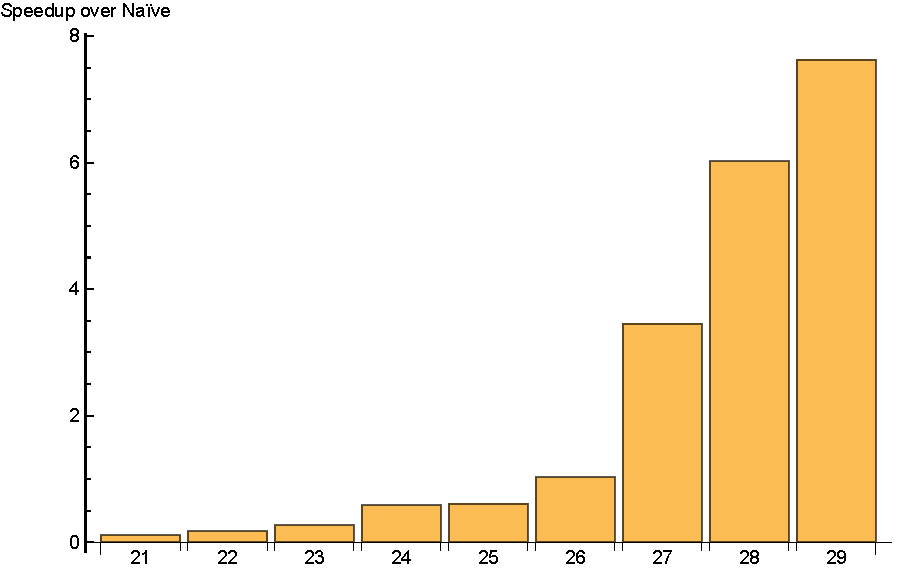
\includegraphics[scale=0.5]{data/stencil.pdf}
\caption{Speedup of convolution over naive CUDA implementation.
	The $x$-axis is the convolved vector size in bytes.}
\label{fig:stencil}
\centering
\end{figure}

Convolutions has wide applications in both engineering and mathematics.
Depending on the ``kernel'' (or mask), convolution, or stencil as it is sometimes called,  	can be used to approximate a differential operator ---
 a $[-\frac{1}{h}, 0, \frac{1}{h}]$ kernel approximates the gradient operator, for example.
High-performance CPU convolution implementations
involve vectorization and tiling to make full use of cache bandwidth and
execution resources.
The biggest impact from a GPU point of view, however, is the use of fast
	scratch pad memory as a user managed cache.
We therefore see little performance benefits from our compiler passes, and the
	performance primarily stems from interleaving memory copies.
Figure~\ref{fig:stencil} shows the speedup achieved by our runtime for a 1D
	convolution compared to a naive CUDA implementation.


\subsection{Option Pricing}

\subsubsection{Black-Scholes}
Black-Scholes models option pricing by simplifying its formula, and some other stuff....


Coarsening increases register pressure, and degrades performance.


\begin{figure}
\centering
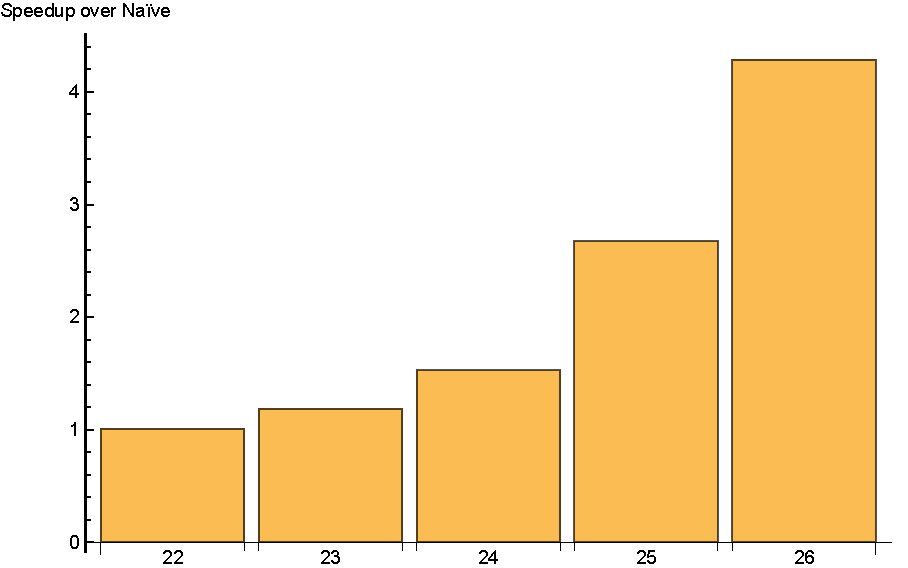
\includegraphics[scale=0.5]{data/blackscholes.pdf}
\caption{Speedup over CUDA version..todo}
\label{fig:blackscholes}
\centering
\end{figure}


\subsubsection{European Options}

\subsection{Binary Image Segmentation}

Binary image segmentation partitions an image into forground and background
	pixels.
We examine the performance of two state of the art algorithms.
The first is GrowCut\todo[inline]{cite} which uses cellular automaton to flood
	neighbors based on an initial seed.
The second uses a graph cut's push-relabel algorithm to find the minimum
	cut to partition the forground and background pixels.

\subsubsection{GrowCut}

\todo[inline]{GrowCut}

\subsubsection{GraphCut}

\todo[inline]{GraphCut}

\subsection{Histogram}

\begin{figure}
\centering
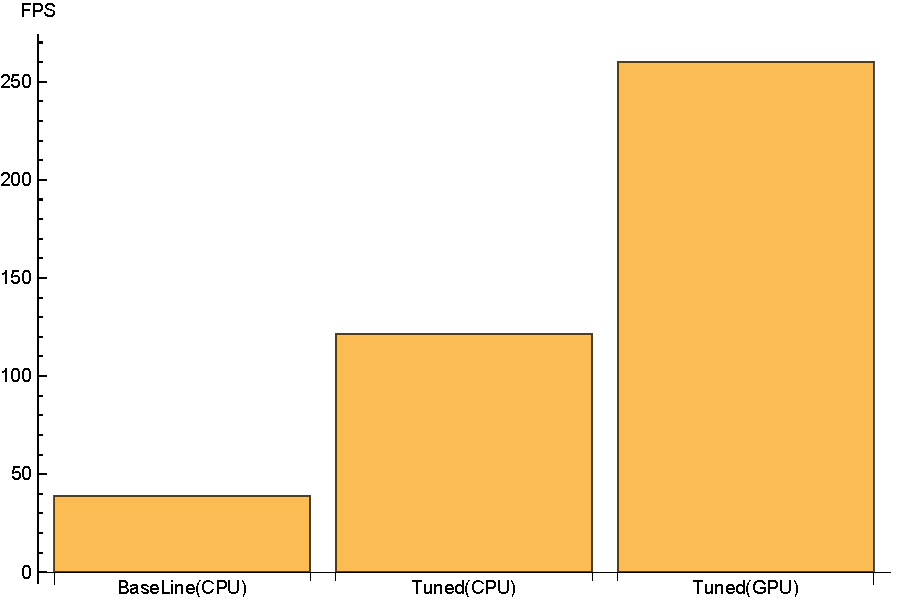
\includegraphics[scale=0.5]{data/histogram.pdf}
\caption{Frames per seconds achieved for histogram equalization kernel on a 4K video. The figure compares the tuned GPU implementation to a naive CPU and tuned CPU implementations. The tuned GPU implementation uses thread coarsening to achieve high fps.}
\label{fig:histogram}
\centering
\end{figure}


\begin{figure}
\centering
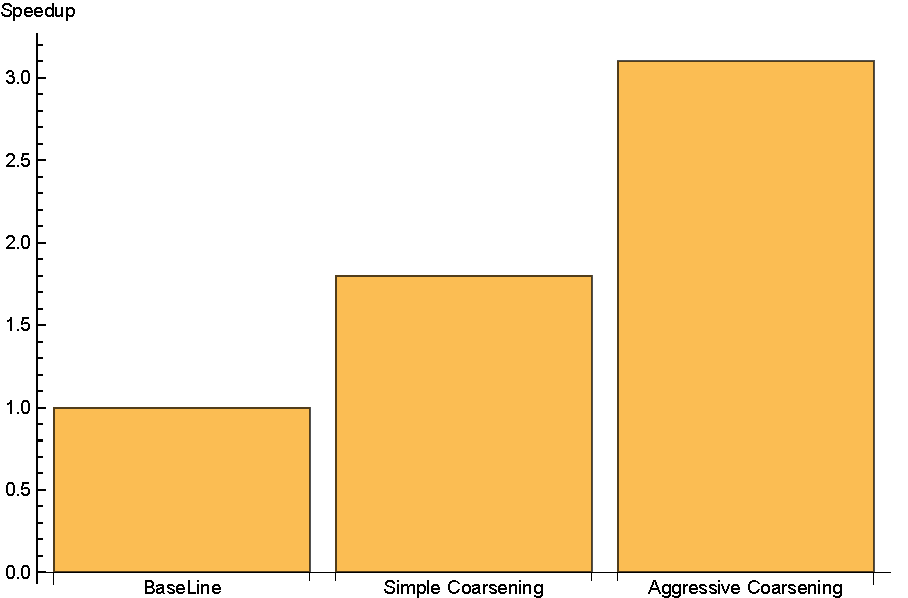
\includegraphics[scale=0.5]{data/histogramc.pdf}
\caption{The coarsening parameter impacts the performance of the histogram equalization kernel.}
\label{fig:histogramCoarsining}
\centering
\end{figure}

Histograms are a fundamental analysis tool in image and data processing.
Efficient serial CPU histogram implementations are very straightforward, but
due to the data-dependent access pattern efficient GPU implementations are
more involved. They typically feature privatization,
where individual histograms for portions of the data are computed separately
and then compiled together into the overall result. This reduces serialization
of atomic memory accesses when different threads increment the same bin.
Other approaches include sorting the input data and then finding the start
index of each bucket, and approaches that use graphics-specific hardware like
occlusion queries.
